\documentclass[]{book}
\usepackage{lmodern}
\usepackage{amssymb,amsmath}
\usepackage{ifxetex,ifluatex}
\usepackage{fixltx2e} % provides \textsubscript
\ifnum 0\ifxetex 1\fi\ifluatex 1\fi=0 % if pdftex
  \usepackage[T1]{fontenc}
  \usepackage[utf8]{inputenc}
\else % if luatex or xelatex
  \ifxetex
    \usepackage{mathspec}
  \else
    \usepackage{fontspec}
  \fi
  \defaultfontfeatures{Ligatures=TeX,Scale=MatchLowercase}
\fi
% use upquote if available, for straight quotes in verbatim environments
\IfFileExists{upquote.sty}{\usepackage{upquote}}{}
% use microtype if available
\IfFileExists{microtype.sty}{%
\usepackage{microtype}
\UseMicrotypeSet[protrusion]{basicmath} % disable protrusion for tt fonts
}{}
\usepackage{hyperref}
\hypersetup{unicode=true,
            pdftitle={The Serpent and the Brain: A Neuroscientific Perspective on Archetypes},
            pdfauthor={Dr.~Dominique Makowski},
            pdfborder={0 0 0},
            breaklinks=true}
\urlstyle{same}  % don't use monospace font for urls
\usepackage{natbib}
\bibliographystyle{apalike}
\usepackage{longtable,booktabs}
\usepackage{graphicx,grffile}
\makeatletter
\def\maxwidth{\ifdim\Gin@nat@width>\linewidth\linewidth\else\Gin@nat@width\fi}
\def\maxheight{\ifdim\Gin@nat@height>\textheight\textheight\else\Gin@nat@height\fi}
\makeatother
% Scale images if necessary, so that they will not overflow the page
% margins by default, and it is still possible to overwrite the defaults
% using explicit options in \includegraphics[width, height, ...]{}
\setkeys{Gin}{width=\maxwidth,height=\maxheight,keepaspectratio}
\IfFileExists{parskip.sty}{%
\usepackage{parskip}
}{% else
\setlength{\parindent}{0pt}
\setlength{\parskip}{6pt plus 2pt minus 1pt}
}
\setlength{\emergencystretch}{3em}  % prevent overfull lines
\providecommand{\tightlist}{%
  \setlength{\itemsep}{0pt}\setlength{\parskip}{0pt}}
\setcounter{secnumdepth}{5}
% Redefines (sub)paragraphs to behave more like sections
\ifx\paragraph\undefined\else
\let\oldparagraph\paragraph
\renewcommand{\paragraph}[1]{\oldparagraph{#1}\mbox{}}
\fi
\ifx\subparagraph\undefined\else
\let\oldsubparagraph\subparagraph
\renewcommand{\subparagraph}[1]{\oldsubparagraph{#1}\mbox{}}
\fi

%%% Use protect on footnotes to avoid problems with footnotes in titles
\let\rmarkdownfootnote\footnote%
\def\footnote{\protect\rmarkdownfootnote}

%%% Change title format to be more compact
\usepackage{titling}

% Create subtitle command for use in maketitle
\providecommand{\subtitle}[1]{
  \posttitle{
    \begin{center}\large#1\end{center}
    }
}

\setlength{\droptitle}{-2em}

  \title{The Serpent and the Brain: A Neuroscientific Perspective on Archetypes}
    \pretitle{\vspace{\droptitle}\centering\huge}
  \posttitle{\par}
    \author{Dr.~Dominique Makowski}
    \preauthor{\centering\large\emph}
  \postauthor{\par}
      \predate{\centering\large\emph}
  \postdate{\par}
    \date{2019-11-13}

\usepackage{booktabs}
\usepackage{amsthm}
\makeatletter
\def\thm@space@setup{%
  \thm@preskip=8pt plus 2pt minus 4pt
  \thm@postskip=\thm@preskip
}
\makeatother

\begin{document}
\maketitle

{
\setcounter{tocdepth}{1}
\tableofcontents
}
\hypertarget{introduction}{%
\chapter{Introduction}\label{introduction}}

Placeholder

\hypertarget{history-of-archetypes}{%
\chapter{History of Archetypes}\label{history-of-archetypes}}

Placeholder

\hypertarget{carl-jung-1875---1961}{%
\section{Carl Jung (1875 - 1961)}\label{carl-jung-1875---1961}}

\hypertarget{philosophical-roots}{%
\section{Philosophical roots}\label{philosophical-roots}}

\hypertarget{archetypal-interpretation-of-the-tarot}{%
\section{Archetypal Interpretation of the Tarot}\label{archetypal-interpretation-of-the-tarot}}

\hypertarget{joseph-campbell-1904---1987}{%
\section{Joseph Campbell (1904 - 1987)}\label{joseph-campbell-1904---1987}}

\hypertarget{robert-moore-1942---2016}{%
\section{Robert Moore (1942 - 2016)}\label{robert-moore-1942---2016}}

\hypertarget{carol-pearson-1944---present}{%
\section{Carol Pearson (1944 - Present)}\label{carol-pearson-1944---present}}

\hypertarget{other-developpments}{%
\section{Other Developpments}\label{other-developpments}}

\hypertarget{a-scientific-archetypism}{%
\chapter{A Scientific Archetypism}\label{a-scientific-archetypism}}

\textbf{\emph{Warning:} This is a work in progress, i.e., currently just a collection of unstructured information.}

\hypertarget{from-theory-to-application}{%
\section{From Theory to Application}\label{from-theory-to-application}}

Following Jung's work, many archetype theorists have adopted a ``bottom-up approach'', i.e., starting from observations to infer the cause (the nature of archetypes). Observations are gathered by exploring various cultures, myths, religions or the depths of Human's psyche (using tools of pseudo-access such as psychoanalysis or hypnosis). In this framework, the archetypist's role is to assemble and integrate the interpretations emerging from these observations, in a theory that could be applied to explain these observations.

In this book, we will take the opposite approach. Based on scientific knowledge about evolution, biology and neuroscience, we will outline a plausible framework, that we will then test on observations and facts.

\hypertarget{a-falsifiable-theory}{%
\section{A Falsifiable Theory}\label{a-falsifiable-theory}}

The fundamental issue of psychoanalysis is that it is not a scientific theory, which requires a possibility of falsification. For example, Newton's law of gravity could easily be falsified if, for instance, the apple did not fall from the tree but levitated there (and it has been later falsified by astronomical observations, and eventually replaced, by Einstein's set of theories). On the contrary, every observation is evidence in favour of psychoanalysis, and the same can unfortunately be said for Jungian's approach.

This pseudoscientific nature is particularly relevant for the Jungian conceptualisation of archetypes, which suffers from a structural and inherent unscientificalness. In metaphorical terms, we could say that it is an \emph{ouroboros} (the symbol of a dragon/serpent eating its own tail): the natural ``consequences'' of archetypes (i.e., the manifest patterns and motifs that we observe in myths, stories, religions\ldots) are also, in theory, the ``cause'' of them. In other words, the existence of numerous instances of wise old men is brandished as the one of the only possible manifest proof for the existence of the archetype of the wise old man. And the redundancy of this motif is also what perpetuates its archetypal nature. The serpent eats itself, and the existence of this archetype, as it is tied only to a given existing observation, is unfalsifiable. On an abstract level, if \emph{B} is the cause of \emph{C}, usually scientists would investigate the cause(s) and origin(s) of \emph{B}, \emph{A}, so that \emph{A} → \emph{B} → \emph{C}.

\begin{figure}
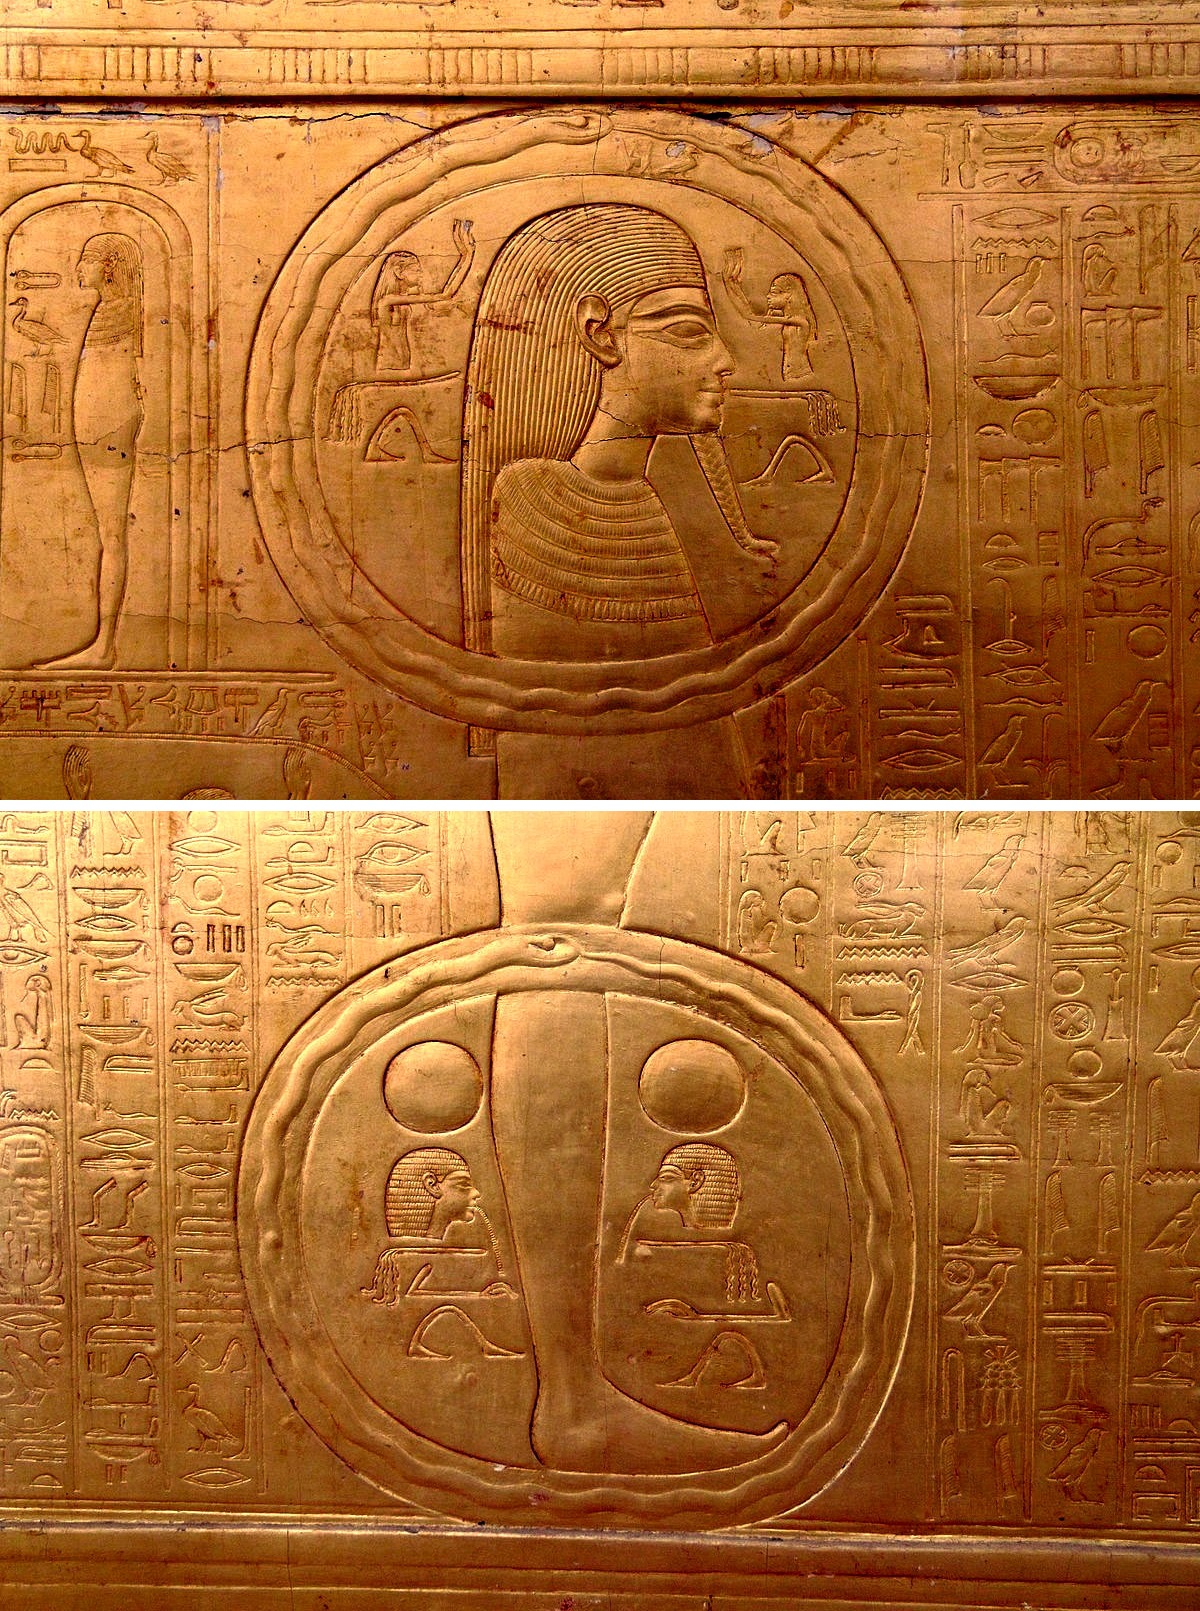
\includegraphics[width=0.49\linewidth]{img/ouroboros_tutankhumon} \caption{The oldest clear depictions of an ouroboros, appearing on the second gilded shrine of Tutankhamun (14th century BC).}\label{fig:unnamed-chunk-1}
\end{figure}

How to scientifically test (and refute) archetypism?

Examples of experiments:

\begin{itemize}
\tightlist
\item
  Child remembers a story and its content where the protagnositc are congruent with archetypes?
\item
  Pseudo-role playing game where participanats have to decide which archetypal character to go ask for specific archetypical questions
\item
  Comparative exploration of proto-religions
\end{itemize}

\hypertarget{limitations}{%
\section{Limitations}\label{limitations}}

Two issues:
- Some data is already known
- Already inspired by existing data

One of the main angle of attacks could be the practical value of generic archetype. Yes, a loving mother and a fearless father are common tropes in Human existence. What is the point of creating a whole pseudo-theory around them? A collateral question would be, do they (as concepts) have any direct influence over our lives?

\hypertarget{definition}{%
\chapter{Definition}\label{definition}}

\textbf{\emph{Warning:} This is a work in progress, i.e., currently just a collection of unstructured information.}

Archetypes are the personification of fundamental lines that structure the psychological system, creating layers of opposed poles tied to important concepts for adaptation and survial. Archetypes are not collective \emph{per se}. They are deeply individual, and their recurrence is merely a reflection of the ontogenical and evolutionary redundancies.

The main archetypes discussed in this chapter reffered to as ``axial archetypes'', as they emerge from to the axes that structure our mental system. As this system grows and complexifies, its dimensionality increases, creating new planes and providing more coordinates to navigate in this space. As a result of the densification of this matrix, archetypes become more subtler, fine-grained and ultimately fading into the unicity that is characterising our identity.

Thus, archetypes are usually paired (as they are the two spaces created separated by a line), creating a symmetric and hierarchical structure. Importantly, they can be identified, and grouped, relative to their causing axis, which is often an important distinction that the organism has to learn in order to adapt.

Thus, evidence for archetypes can be indirectly gathered by demonstrating the existence and relevance of their axis of reference.

\hypertarget{the-main-archetypes}{%
\chapter{The Main Archetypes}\label{the-main-archetypes}}

Placeholder

\hypertarget{masculine-and-feminine}{%
\section{Masculine and Feminine}\label{masculine-and-feminine}}

\hypertarget{the-two-worlds}{%
\section{The Two Worlds}\label{the-two-worlds}}

\hypertarget{known-vs.-unknown}{%
\section{\texorpdfstring{Known \emph{vs.} Unknown}{Known vs. Unknown}}\label{known-vs.-unknown}}

\hypertarget{time}{%
\section{Time}\label{time}}

\hypertarget{moral}{%
\section{Moral}\label{moral}}

\hypertarget{order}{%
\section{Order}\label{order}}

\hypertarget{death}{%
\section{Death}\label{death}}

\hypertarget{the-artist}{%
\section{The artist}\label{the-artist}}

\hypertarget{the-serpent}{%
\section{The Serpent}\label{the-serpent}}

\hypertarget{light-and-shadow}{%
\section{Light and Shadow}\label{light-and-shadow}}

\hypertarget{archetypes-and-psychology}{%
\chapter{Archetypes and Psychology}\label{archetypes-and-psychology}}

\textbf{\emph{Warning:} This is a work in progress, i.e., currently just a collection of unstructured information.}

The archetypal framework developped in this book is by essence reductionist, exploring the abstract core features of cognition and essentializing them to concepts of pure abstraction. As such, archetypes do not directly relate to individual psychology, nor to anything tangible.

\hypertarget{archetypes-as-heuristics}{%
\section{Archetypes as Heuristics}\label{archetypes-as-heuristics}}

One could define an archetype is a basic frame facilitating a basic, instinctive, and intuitive understanding of a concept or a personality. This definition brings it close to a key concept in psychology, heuristics.

\hypertarget{relationship-with-personality}{%
\section{Relationship with Personality}\label{relationship-with-personality}}

\hypertarget{archetypes-and-the-brain}{%
\chapter{Archetypes and the Brain}\label{archetypes-and-the-brain}}

\textbf{\emph{Warning:} This is a work in progress, i.e., currently just a collection of unstructured information.}

Do archetypes have a biological existence?

\hypertarget{origin}{%
\section{Origin}\label{origin}}

Are the archetypes innate? No, (altough they might have been favoured by evolution); they stem out of the redunduncies of existence.

\hypertarget{archetypes-as-neurocognitive-invariants}{%
\section{Archetypes as Neurocognitive Invariants}\label{archetypes-as-neurocognitive-invariants}}

contrary to Jung, these archetypes are not originating from some collective unconscious, but rather are created and maintained by the ontology of the individual, and patterns are crystilised out of the répétition and similarity accross individual ontologies (e.g., the presnece of a fatherly and a motherly figure, etc.)

\hypertarget{neurological-substrate}{%
\section{Neurological Substrate}\label{neurological-substrate}}

Attempts have been made to map archetypes unto brain structures \citep{samuels2003jung}. For instance, \citet{rossi1977cerebral} suggested that one could locate the archetypes in the right cerebral hemisphere, based on the idea that the left hemisphe would be primarily verbal and associational, and the right primarily visuospatial and apperceptive. In light of the current neuroscientific data, these theories appear as nonsensical and naive.

That being said, if archetypes are engrammed into the cognitive system, a biological basis has to exist. One potential answer is to reframe archetypism under the predictive coding framework. As such, archetypes could be seen as meta-priors.

\hypertarget{archetypal-stories}{%
\chapter{Archetypal stories}\label{archetypal-stories}}

\textbf{\emph{Warning:} This is a work in progress, i.e., currently just a collection of unstructured information.}

Common motives in religions and myths beg the question of the existence or plausibility of archetypal stories.

\hypertarget{the-origin-of-religions}{%
\chapter{The Origin of Religions}\label{the-origin-of-religions}}

Placeholder

\hypertarget{history-of-cosmos-conceptualisations}{%
\section{History of Cosmos-Conceptualisations}\label{history-of-cosmos-conceptualisations}}

\hypertarget{scientific-theories-of-religion}{%
\section{Scientific Theories of Religion}\label{scientific-theories-of-religion}}

\hypertarget{evolutionary-perspective}{%
\subsection{Evolutionary Perspective}\label{evolutionary-perspective}}

\hypertarget{cognitive-perspective}{%
\subsection{Cognitive Perspective}\label{cognitive-perspective}}

\hypertarget{neuro-ontogenical-perspective}{%
\subsection{Neuro-ontogenical Perspective}\label{neuro-ontogenical-perspective}}

\hypertarget{proto-beliefs-vs.-religion}{%
\section{Proto-beliefs vs.~Religion}\label{proto-beliefs-vs.-religion}}

\hypertarget{the-symbolic-of-elements}{%
\section{the symbolic of elements}\label{the-symbolic-of-elements}}

\bibliography{book.bib,packages.bib}


\end{document}
